Coaxial cables are one of the major types of cables which are commonly used. First invented for telegraph transmission in 1880 as patient number 1407 (1,800,000 patients are filed per year now) by Oliver Heaviside, it is still one of the main cable types used widely for connecting the world, with the widest deployment of coaxial cables for television and internet distribution. The Coaxial cable have inbuilt characteristics which significantly affect the signals which they propagate and we set out to measure these characteristics in this lab.
\\

A Coaxial cable is named as it has layers of conductors throughout its axis, it is layered in four distinct layers, the center is a conductive wire, then a dielectric layer around it, with another conductive layer around that for shielding purposes and finally a insulating layer for protection. These layers can be seen in Figure \ref{fig:Cable}.

\begin{figure}[H]
\centering
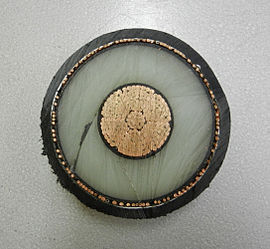
\includegraphics[width=0.25\textwidth]{figures/Coaxial_cable.jpg}
\caption{Coaxial cable split across to show the layers. \cite{pict_cable}}
\label{fig:Cable}
\end{figure}

\\
Through the cables we transmit electricity, and noting that we are interested in transmitting Alternating Current (AC) through the cables, so consideration of the signals as waves is necessary, and through the characteristics of these waves and we will be able to derive characteristics of the cables.

\\

In this paper we will first outline the coaxial cable as a wave guide, and from this we will be able to relate the dieletric layer's characteristic electric permittivity to physically measurable quantities. Then we will be able to define a procedure for investigating these properties and some other properties for the characterization of the cable, which will lead us to determine the material of the cable through its permittivity. 